\section{Experimentación y resultados}
\label{sec:experimentacion}

\subsection{Diseño experimental común}

Todos los experimentos comparten un protocolo de rigor: (i) \emph{igualdad de presupuesto} entre métodos comparados; (ii) múltiples semillas de ejecución (5 en todos los casos) con media, desviación típica muestral (división por $n-1$) y curvas de convergencia con banda de una desviación; (iii) fitness robusto en CartPole: cada evaluación usa condiciones iniciales nuevas, sorteadas con semillas preasignadas; (iv) separación estricta entrenamiento/validación/test en la vertiente UCI. Las figuras se regeneran íntegramente con los scripts de \texttt{experiments/} (verificado: los tres experimentos de NumPy reproducen bytes idénticos en cualquier máquina).

\subsection{Coste computacional: speedup de la evaluación paralela}

Se cronometra la misma tarea de evaluación de poblaciones de 50 redes $(4,16,16,2)$ con 5 repeticiones por configuración, en una máquina de 12 núcleos, con calentamiento previo de los procesos. Dos cargas de trabajo: \emph{ligera} (población aleatoria, episodios de $\approx$10 pasos) y \emph{pesada} (población evolucionada que sobrevive episodios completos, la situación real de las generaciones tardías).

\begin{table}[htbp]
  \centering
  \caption{Tiempo medio por población (s) y aceleración frente al secuencial.}
  \label{tab:speedup}
  \begin{tabular}{lcccccc}
    \toprule
    Procesos & 1 & 2 & 4 & 8 & 12 & \\
    \midrule
    Población aleatoria (s) & 0,251 & 0,156 & 0,096 & 0,079 & 0,086 & \multicolumn{1}{r}{(sec.: 0,226)} \\
    Aceleración & 0,90$\times$ & 1,45$\times$ & 2,36$\times$ & 2,85$\times$ & 2,63$\times$ & \\
    Población evolucionada (s) & 2,320 & 1,285 & 0,851 & 0,559 & 0,475 & \multicolumn{1}{r}{(sec.: 2,264)} \\
    Aceleración & 0,98$\times$ & 1,76$\times$ & 2,66$\times$ & 4,05$\times$ & \textbf{4,76$\times$} & \\
    \bottomrule
  \end{tabular}
\end{table}

\begin{figure}[htbp]
  \centering
  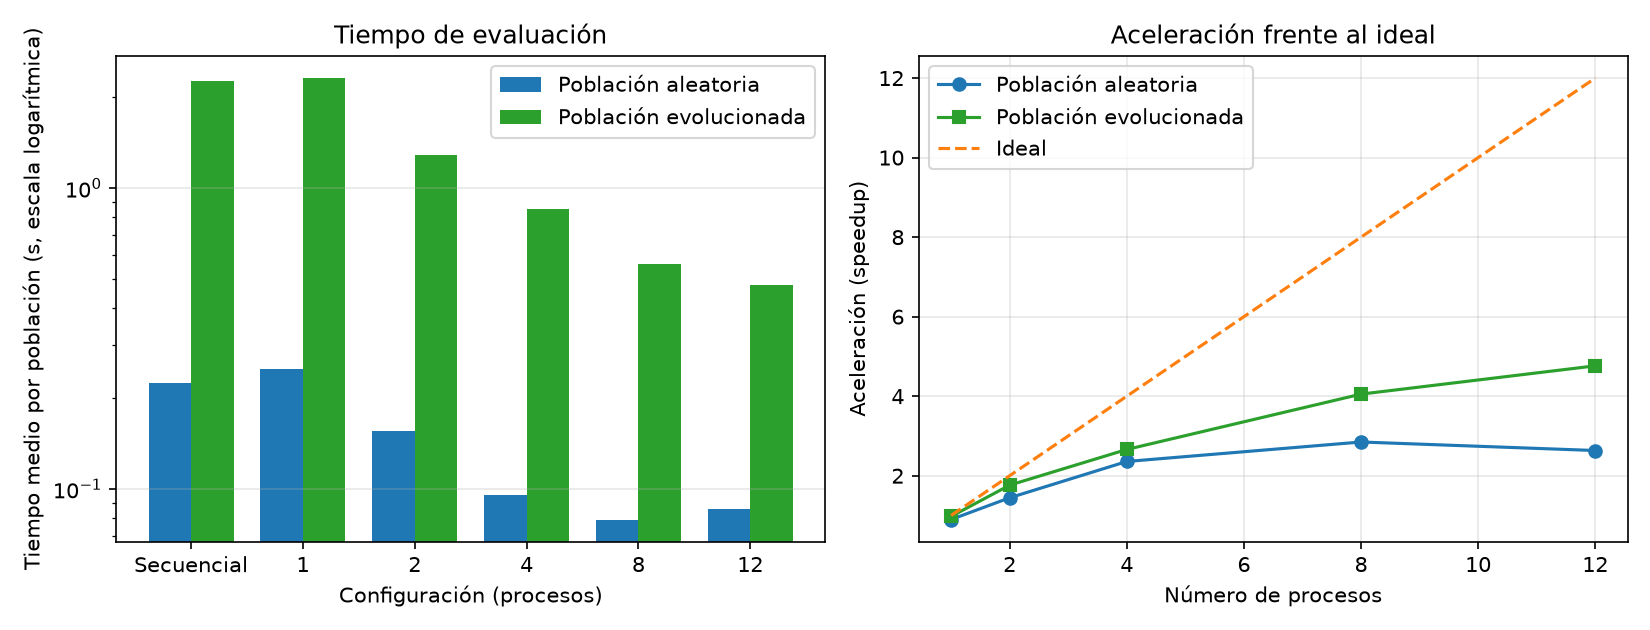
\includegraphics[width=0.95\linewidth]{parallel_speedup.png}
  \caption{Tiempo de evaluación (izquierda, escala logarítmica) y aceleración frente al ideal (derecha) para cargas ligera y pesada.}
  \label{fig:speedup}
\end{figure}

La carga pesada alcanza \textbf{4,76$\times$ con 12 procesos}, mientras la ligera se estanca en 2,85$\times$ y empeora a 12 (2,63$\times$): cuando cada tarea dura milisegundos, la coordinación entre procesos supera al trabajo ahorrado. Ninguna curva llega a la ideal $S(p)=p$ por (a) el coste de serializar cromosomas y recoger resultados y (b) la ley de Amdahl: la parte no paralelizable (creación de población, selección, cruce, mutación) limita el máximo. Con un trabajador el pool cuesta prácticamente nada (0,90--0,98$\times$), lo que confirma que la medición ya no incluye el arranque de procesos.

\subsection{CartPole: algoritmo genético frente a búsqueda aleatoria}

Con la red $(4,16,16,2)$, población 50, 3000 evaluaciones y 5 semillas (figura~\ref{fig:cartpole}):

\begin{table}[htbp]
  \centering
  \caption{Resultados en CartPole-v1 (5 semillas, 3000 evaluaciones).}
  \label{tab:cartpole}
  \begin{tabular}{lccc}
    \toprule
    Método & Mejor final (media $\pm$ dt) & Éxito (500) & Evaluaciones hasta 500 (media $\pm$ dt) \\
    \midrule
    Algoritmo genético & 500,0 $\pm$ 0,0 & 5/5 & 470 $\pm$ 317 \\
    Búsqueda aleatoria & 487,2 $\pm$ 28,6 & 4/5 & 700 $\pm$ 402 \\
    \bottomrule
  \end{tabular}
\end{table}

\begin{figure}[htbp]
  \centering
  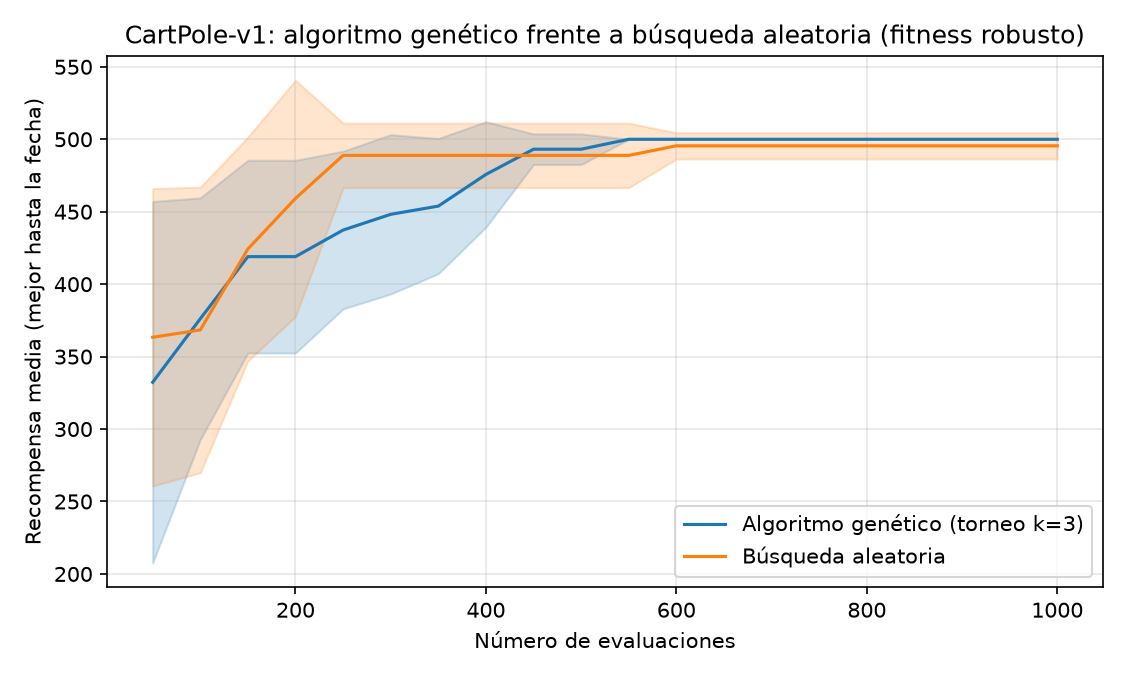
\includegraphics[width=0.85\linewidth]{phase1_ga_vs_random.png}
  \caption{CartPole-v1 (red 4-16-16-2): mejor hasta la fecha frente a evaluaciones, media de 5 semillas con banda de una desviación típica.}
  \label{fig:cartpole}
\end{figure}

El AG resuelve las 5 semillas y llega al óptimo $\approx$1,5$\times$ antes que la búsqueda aleatoria entre las ejecuciones exitosas. Dato preliminar relevante para la discusión: con la red \emph{pequeña} de 58 pesos, la búsqueda aleatoria saturaba el entorno (bastaba con suerte para estabilizar el polo), por lo que el protocolo se endureció con fitness robusto y una red mayor.

\subsection{Comparación de operadores genéticos}

Cuatro configuraciones (selección $\times$ cruce) con 5 semillas y 3000 evaluaciones cada una, todo lo demás idéntico:

\begin{table}[htbp]
  \centering
  \caption{Evaluaciones hasta la puntuación perfecta (media $\pm$ dt sobre las 5 semillas).}
  \label{tab:operadores}
  \begin{tabular}{lccc}
    \toprule
    Configuración & Éxito & Hasta 500 & Mejor final \\
    \midrule
    Ruleta + cruce un punto & 5/5 & \textbf{220 $\pm$ 220} & 500 $\pm$ 0 \\
    Torneo + BLX-$\alpha$ & 5/5 & 310 $\pm$ 290 & 500 $\pm$ 0 \\
    Torneo + cruce un punto & 5/5 & 470 $\pm$ 317 & 500 $\pm$ 0 \\
    Torneo + cruce uniforme & 5/5 & 550 $\pm$ 580 & 500 $\pm$ 0 \\
    \bottomrule
  \end{tabular}
\end{table}

\begin{figure}[htbp]
  \centering
  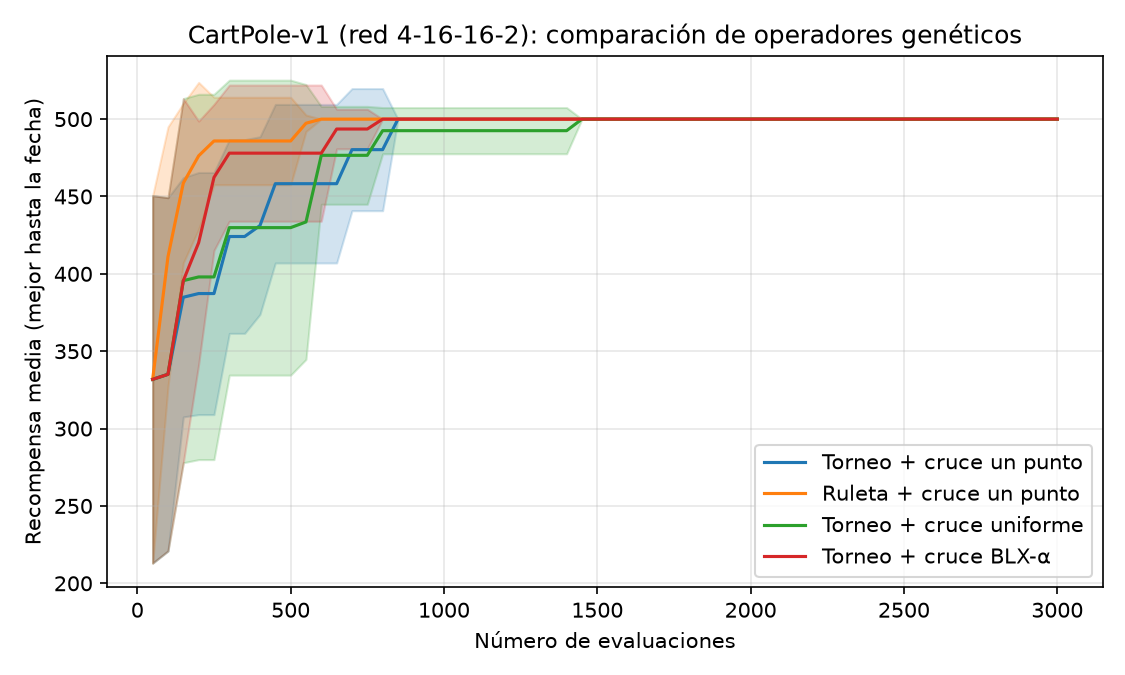
\includegraphics[width=0.85\linewidth]{operator_comparison.png}
  \caption{Comparación de operadores genéticos en CartPole-v1 (red 4-16-16-2).}
  \label{fig:operadores}
\end{figure}

Todas las configuraciones saturan la tarea, así que la discriminación está en la \emph{eficiencia}: la ruleta alcanza el óptimo antes que el torneo en \emph{todas} las semillas (4 victorias y 1 empate por parejas), seguida de BLX-$\alpha$, que confirma la ventaja teórica de muestrear en torno a los progenitores para pesos reales; el cruce uniforme, que destroza bloques de genes coadaptados, es el más lento y el más variable. La ausencia de estancamiento de la ruleta se explica porque el fitness es ruidoso (nadie puede monopolizar la selección) y el elitismo protege al mejor sin depender de la selección.

\subsection{Comparación a igual presupuesto de episodios: AG, aleatoria y REINFORCE}

Las tres compiten con el mismo presupuesto de 9000 episodios (el AG y la aleatoria lo consumen como 3000 evaluaciones $\times$ 3 episodios; REINFORCE entrena 9000 episodios), sobre un eje común de episodios jugados:

\begin{table}[htbp]
  \centering
  \caption{Comparación con igual presupuesto de 9000 episodios (5 semillas).}
  \label{tab:tresmetodos}
  \begin{tabular}{lccc}
    \toprule
    Método & Éxito (500) & Episodios hasta 500 & Mejor final \\
    \midrule
    Algoritmo genético & 5/5 & \textbf{1261 $\pm$ 952} & 500,0 $\pm$ 0,0 \\
    Búsqueda aleatoria & 5/5 & 2791 $\pm$ 2198 & 500,0 $\pm$ 0,0 \\
    REINFORCE ($\nu = 0{,}001$) & 3/5 & 3933 $\pm$ 1511 & 464,2 $\pm$ 70,9 \\
    \bottomrule
  \end{tabular}
\end{table}

\begin{figure}[htbp]
  \centering
  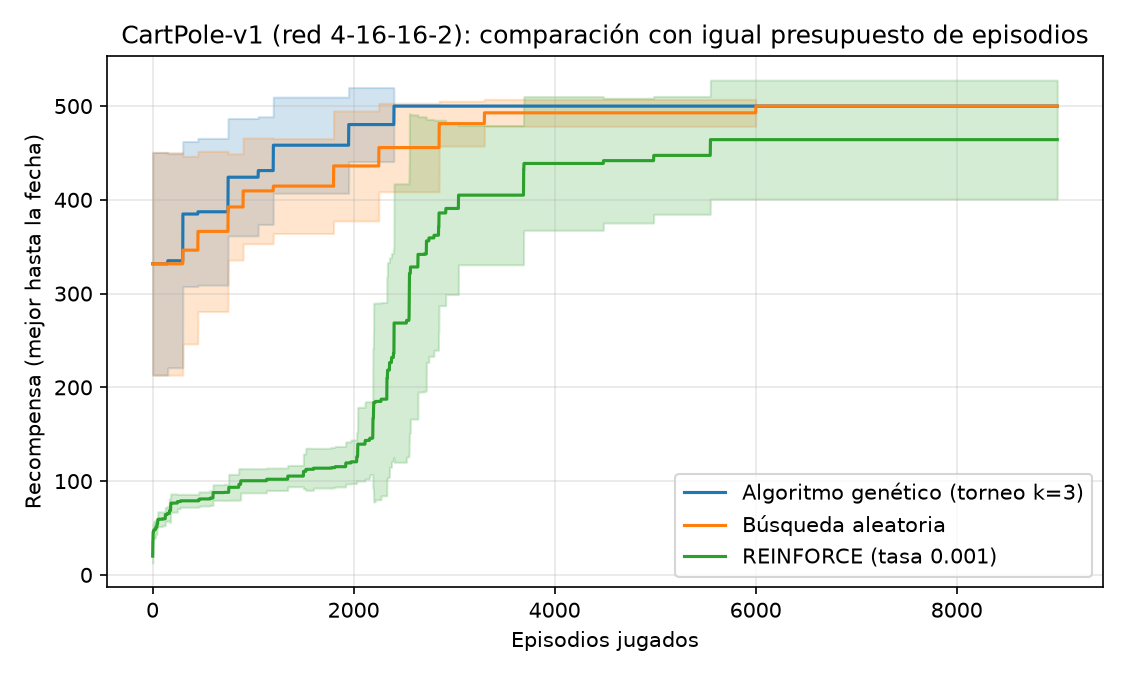
\includegraphics[width=0.85\linewidth]{reinforce_comparison.png}
  \caption{Comparación con igual presupuesto de episodios en CartPole-v1 (red 4-16-16-2).}
  \label{fig:tresmetodos}
\end{figure}

El AG alcanza el óptimo con \textbf{2,2}$\times$ menos episodios que la aleatoria y \textbf{3,1}$\times$ menos que REINFORCE, y es el único método fiable en todas las semillas. La curva de REINFORCE muestra su patrón clásico: meseta inicial $\approx$100 pasos durante 2000 episodios, despegue entre 2200 y 3500 y techo con banda muy ancha (alto sesgo de varianza del estimador de política). Con la tasa $0{,}01$ aprobada inicialmente la política \emph{colapsaba}; la sonda con $10^{-3}$ fue la más rápida que aprende de forma estable.

\subsection{Letter Recognition: arquitectura e hiperparámetros}

Presupuesto de 240 evaluaciones por semilla (población 20, 20 épocas de entrenamiento cada evaluación, 8 procesos), fitness en validación y evaluación final en test:

\begin{table}[htbp]
  \centering
  \caption{Exactitud (media $\pm$ dt, 5 semillas) en Letter Recognition.}
  \label{tab:letter}
  \begin{tabular}{lccc}
    \toprule
    Método & Validación & Test & Tiempo medio de búsqueda \\
    \midrule
    Algoritmo genético & \textbf{0,9619 $\pm$ 0,0044} & \textbf{0,9612 $\pm$ 0,0098} & 637,9 s \\
    Búsqueda aleatoria & 0,9501 $\pm$ 0,0079 & 0,9540 $\pm$ 0,0096 & 561,7 s \\
    Configuración por defecto (1 ejec.) & 0,8733 $\pm$ 0,0021 & 0,8856 $\pm$ 0,0036 & --- \\
    \bottomrule
  \end{tabular}
\end{table}

\begin{figure}[htbp]
  \centering
  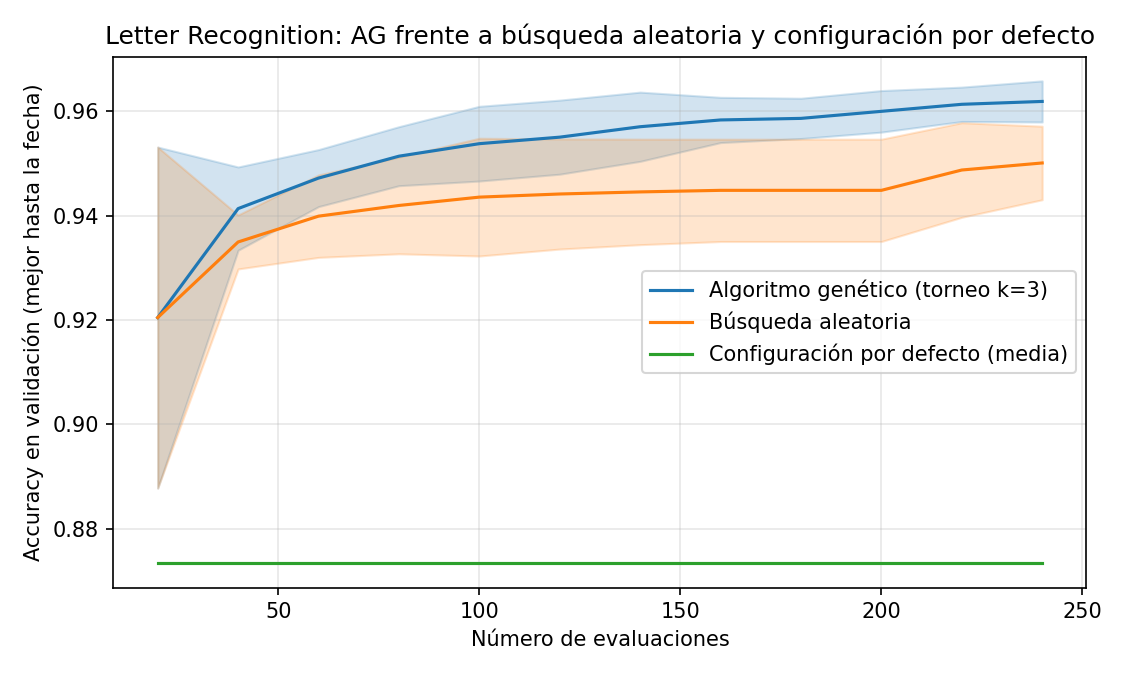
\includegraphics[width=0.85\linewidth]{phase3_ga_vs_random.png}
  \caption{Letter Recognition: AG frente a búsqueda aleatoria y a la configuración por defecto (media de validación).}
  \label{fig:letter}
\end{figure}

El AG supera a la búsqueda aleatoria en validación en \emph{todas} las semillas (5/5 por parejas) y ambos superan ampliamente a la configuración por defecto (8--9 puntos porcentuales). En test la ventaja del AG se reduce a 0,7--1,2 puntos con desviaciones de $\approx$1 punto: la comparación honesta es la de test (ver discusión). La re-ejecución íntegra en otra máquina reprodujo las conclusiones con diferencias de cuarto decimal, atribuibles a la no-exactitud de las rutinas BLAS de PyTorch entre hardware distinto (la versión canónica de la figuras~\ref{fig:letter} y su log es la del repositorio).
